% !TEX root = ../main.tex

\section{Background}
\label{section:background}

To build up to our approach, we use a traditional statistical framework as a guideline for multilabel classificaton methods~\citep{tukey}. We distinguish the desired theoretical statistic (the \textbf{estimand}), its functional form (the \textbf{estimator}) and its approximation (the \textbf{estimate}); the latter estimates can be benchmarked with \textbf{metrics}. We show how multilabel reductions tend to reformulate the estimand and treat labels independently (i.e. change our assumptions about the data). However, with a proper estimator, it is possible to directly model the estimand. Our proposed loss function, \emph{sigmoidF1}, accommodates for the true estimand.

We define a learning algorithm $\mathcal{F}$ (i.e. a class of estimators) that maps inputs to outputs given a set of hyperparameters \(\mathcal{F}(\cdot ; \Theta): \mathcal{X} \rightarrow \mathcal{Y}\). We consider a particular case, with the input vector \(\mathbf{x} = \{x_1, \ldots, x_n\}\) and each observation is assigned $k$ labels (one or more) \(\mathbf{l} = \{l_1, \ldots, l_C\}\) out of a set of $C$ classes. \(y_{i}^{j}\) are binary variables, indicating presence of a label for each observation \(i\) and class \(j\). Together they form the matrix output $\mathbf{Y}$.

\subsection{Estimand and definition of the risk}
\label{section:background:estimand}

We distinguish between two scenarios: the \emph{multiclass} and the \emph{multilabel} scenario. 
In the multiclass scenario, a single example is attributed one class label (e.g., classification of an animal on a picture). 
In the multilabel scenario, a single example can be assigned more than one class label (e.g., movie genres). 
%Multiclass classification deserves a mention towards the end, as it illustrates a straightforward relationship between estimand-estimator-estimate. 
We focus on the multilabel scenario. More formally, for a particular set of input $\mathbf{x}$ (e.g. paper abstracts) and output $\mathbf{Y}$ (e.g. scientific field(s) ) its risk formulation can be written as in ~\citep{multilabelReduction}:
%
\begin{equation}
R_{\mathrm{ML}}(\mathcal{F}) = \mathbb{E}_{(\mathbf{x}, \mathbf{Y})}\left[\mathcal{L}_{\mathrm{ML}}(\mathbf{Y}, \mathcal{F}(\mathbf{x}))\right].
\end{equation}
%
We define $\mathcal{F}$ as the estimand: the theoretical statistic. For one item $x_i$, the theoretical risk defines how close the estimand can get to that deterministic output vector $\mathbf{y}_{i}$.

\if0
For example, corn ($x_{corn}$) is eaten by a finite number of animals that can digest it ($\mathbf{y}_{corn} = {y_{corn}^{horse}, \ldots, y_{corn}^{sheep}} $), assuming animals belong to a finite set of living beings. If one were to predict which food is eaten by which animals, the theoretical risk (estimand) defines how close we can get to that deterministic vector $\mathbf{y}_{corn}$, given $x_{corn}$.
\fi

In practice, statistical models do output probabilities $\mathbf{\hat{y}}_{i}$ via an estimator and its estimate (also called propensities or suitabilities~\citep{multilabelReduction}). The solution to that stochastic-deterministic incompatibility is either to convert the estimator to a deterministic measure via decision thresholds (e.g. traditional cross-entropy loss), or to treat the estimand as a stochastic measure (our sigmoidF1 loss proposal).

\subsection{Estimator: the functional form}
\label{section:background:estimator}

The estimator $f \in \mathcal{F}$ is any minimizer of the risk $R_{ML}$. Predicting multiple labels per example comes with the assumption that labels are non-mutually exclusive.

\vspace{-.5\baselineskip}
\begin{proposition}
  The multilabel estimator of $y_{i}^{j}$ is dependent on the input and other groundtruth labels for that example,
%
\begin{equation}
  \hat{y}_i^j = f(x, y_{i}^{1}, \ldots, y_{i}^{j-1}) = P(y_i^j = 1 | x, y_{i}^{1}, \ldots, y_{i}^{j-1})
\end{equation}
\label{eq:estimator}
\end{proposition}
\vspace{-1.5\baselineskip}
%
 By proposing this general formulation, we entrench that characteristic in the estimator. Contrary to \citet{multilabelReduction}, our proposal above models interdependence between labels and deals with thresholding for the estimate at training time for free.


\subsection{Estimate: approximation via a loss function}
\label{section:background:estimate}

Most of the literature found on multilabel classification can be characterized as multilabel reductions~\cite{multilabelReduction}. Given the general non-convex optimization context, the surrogate loss function $\mathcal{L}(\mathbf{y}_i, f)$ can take different forms\footnote{Note that OVA and PAL have each a form normalised by the number of positive labels~\cite{multilabelReduction}. We leave out pick-one-label, as it is further removed from our discussion.}. 

\subsubsection*{One-versus-all (OVA)}
OVA consists of a reformulation of the multilabel classification task to a sequence of $C$ binary classifications ($f^1, \ldots, f^C$), with $C$ the number of classes:
%
\begin{equation}
\begin{aligned}
\mathcal{L}_{\mathrm{OVA}}(\mathbf{y}_i, f) &= \sum_{c = 1}^C \mathcal{L}_{\mathrm{BC}}\left(y_i^{c}, f^{c}\right)\\
&=\sum_{c = 1}^C \left\{y_{i}^c \cdot \mathcal{L}_{\mathrm{BC}}\left(1, f^c \right)+\left(1-y_{i}^c \right) \cdot \mathcal{L}_{\mathrm{BC}}\left(0, f^c \right)\right\}
\end{aligned}
\end{equation}
%
where $\mathcal{L}_{\mathrm{BC}}$ is a binary classification loss (binary relevance \cite{OVA1, hammingLoss, OVA2}), most often logistic loss.  Note that minimizing binary cross-entropy is equivalent to maximizing for log-likelihood~\cite[\S4.3.4]{Bishop}.

\subsubsection*{Pick-all-labels (PAL)}
The loss function set here is
%
\vspace{-0.5\baselineskip}
\begin{equation}
\mathcal{L}_{\mathrm{PAL}}(\mathbf{y}_i, f) = \sum_{c = 1}^C y_{i}^c \cdot \mathcal{L}_{\mathrm{MC}}(y_i^c, f),
\end{equation}
%
with $\mathcal{L}_{MC}$ a multiclass loss (e.g. softmax cross-entropy). In this formulation, each example $(x_i, \mathbf{y}_i)$ is converted to a multiclass framework, with one observation per positive label. The sum of inherently multiclass losses is used to represent the multilabel estimand. Note that cross-entropy loss can be formulated as \(\mathcal{L}_{\text {CE}}=-\sum \log \left(f \right)\).

\vspace{\baselineskip}

Multilabel reduction methods are characterized by their way of reformulating the estimand, the resulting estimator and the estimate. This allows the use of existing losses: logistic loss (for binary classification formulations), sigmoid loss or softmax cross-entropy loss (for multiclass formulations). These reductions imply a reformulation of the estimator (a.k.a. Bayes Optimal) as follows:
%
\begin{equation}
  \hat{y}_i^j = f(x) = P(y_i^j = 1 | x_i)
\end{equation}
%
Contrary to our definition of the original multilabel estimator (Eq.~\ref{eq:estimator}), independence of label propensities is assumed. In other words the loss function becomes any monotone transformation of the marginal label probabilities $P(y_i^j = 1 | x)$ ~\cite{OVA2, multilabelMetrics, unifiedView}.

% \citet{multilabelReduction} show that OVA, PAL and their normalized counterparts are consistent~\citep{consistency-surrogates, consistency-multiclassSVM, consistency-lossAnalysis} with either precision or recall. A learning algorithm is defined as consistent if the expected risk given $f$ and $\mathcal{L}$ approximates the original estimator (Bayes risk), as the input sample size grows~\cite{consistencyMultilabel}.

\subsection{Metrics: evaluation at inference time}
\label{section:background:metrics}

There is a consensus around the use of confusion matrix  and ranking metrics to evaluate multilabel classification models (at inference time)~\cite{multilabelMetrics, weightedMetrics, unifiedView}. Notably Precision and Recall. Confusion matrix metrics come with caveats: most of these measures 
\begin{enumerate*}
\item require a hard thresholding, and that makes them non-differentiable for Stochastic Gadiant Descent, 
\item they are very sensitive to the choice of the number top labels to include $k$\footnote{In the case of unilabel prediction, top-k becomes a top-1 problem, which essentially eliminates caveats I and II.} ~\cite{decisionThreshold} and 
\item they require aggregation choices to be made in terms of micro / macro / weighted metrics.
\end{enumerate*}
Some common confusion matrix metrics are Precision, Recall, F1-score, hinge-loss or one-error-loss. Numerous others can be formulated~\cite{unifiedView}.


\subsection{Multilabel estimate: F1 Metric as a Loss}
\label{section:background:metricsAsLosses}


In a number of retrieval tasks, a model's out of sample accuracy is measured on metrics such as AUROC, F1 score, etc. These reflect an objective catered towards evaluating the model over an entire ranking. Due to the lack of differentiability, these metrics cannot be directly used as loss functions at training time (in-sample). A seminal Study~\cite{optimizableLosses} derived a general framework for deriving decomposable surrogates to some of these metrics. We propose our own decomposable surrogates tailored for the problem at hand.

In a typical machine learning classification task, binary labels are compared to a probabilistic measure (or a reversible
transformation of a probabilistic measure such as a sigmoid or a softmax
function). If the number $n_i$ of labels to be predicted per
example is known a priori, it is natural at training time to assign the $top_{n_i}$ predictions
to that example~\cite{lossTopKError, topKmulticlassSVM}. If the number of
labels per example is not known a priori, the question remains at both training and at inference time
as to how to decide on the number of labels to assign to each
example. This is generally done via a \emph{decision threshold}, that can be set globally for all
examples. This threshold can optimize for specificity or
sensitivity~\cite{decisionThreshold}. We propose an approach where this threshold is implicitly defined, by using a loss function that penalizes explicitly for wrong label counts and fits to the original estimand in Proposition 1.

That loss function is a surrogate of the F1 score, the harmonic mean of precision and recall (formal definition below). It implicitly deals with label counts and label predictions by including confusion matrix count data. It also balances precision and recall. In the next section, we show how $F_1$ is formulated into a surrogate loss $\mathcal{L}_{\widetilde{\mathit{F1}}}$.



% \begin{figure}[t]
% \centering
% 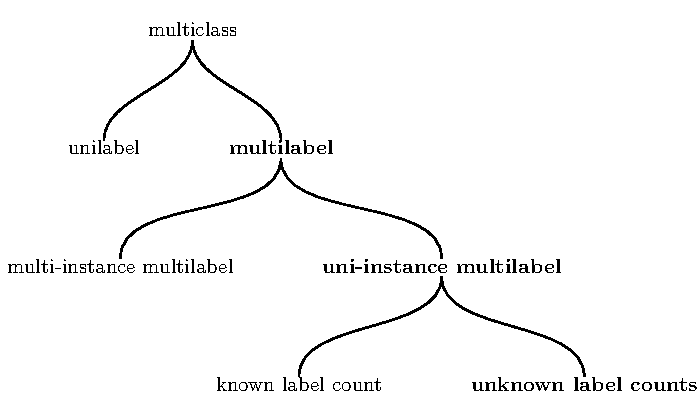
\includegraphics[width=.9\linewidth]{./tree/Tree.pdf}
% \caption{\label{fig:tree} SIMPUL (bold) within the \emph{multiclass}
% nomenclature
% \hvk{figure is not referenced in text, bold is unclear in figure}
% \daan{I think it should go. And if it stays: uni -> single.}
% % Clarifying ``multiclass'' classification problems. In this paper we focus on
% % the uni-instance, multilabel, multiclass classification problem with a
% % varying number of labels (the bottom right hand side of the tree).
% }
% \end{figure}% \mdr{Image source ...}

%%% Local Variables:
%%% mode: latex
%%% TeX-master: "../main"
%%% End: